\documentclass[a4paper,12pt]{article}
\usepackage[russian]{babel}   
\usepackage[utf8]{inputenc}  
\usepackage{xypic}
\usepackage{amssymb}
\usepackage{amsmath}
\usepackage{enumerate}
\usepackage{titlesec}
\usepackage[left=30mm, top=20mm, right=20mm, bottom=17.5mm, nohead, footskip=10mm]{geometry} % настройки полей документа
\usepackage{indentfirst}
\usepackage{setspace}
\usepackage{graphicx}
\graphicspath{{pics/}}
\DeclareGraphicsExtensions{.png}

\singlespacing

\begin{document}
    \section{Введение}
        Дадим некоторые базовые определения.
        Абелевой группой будем называть множество $G$ с определенной на нем операцией $+$ для которого выплонены следующие аксиомы:
        \begin{enumerate}
            \item $\forall a, b \in G$ $a + b \in G$
            \item $\exists 0 : a + 0 = 0 + a \in G$
            \item $\forall a \in G$ $\exists -a \in G : a + (-a) = 0$
            \item $\forall a, b \in G$ $a + b = b + a$
            \item $\forall a, b, c \in G$ $a + (b + c) = (a + b) + c$
        \end{enumerate}
        Проще говоря группой назовем множество элементы которого можно складывать, 
        вычитать и в котором имеется нейтральный элемент относительно данной операции.

        Предположим что мы сейчас работаем в $\mathbb{R}^2$.
        Дадим общее определение того что такое эллиптическая кривая. \textit{Эллиптической кривой} назовем множество точек $(x, y)$,
        удовлетворяющих уравнению $y^2 + a_1xy+a_3y = x^3+a_2x^2+a_4x + a_5$, где $a_i$ -- некоторый числа.
        Множество таких точек обозначим как 
        $$
            E = \{(x, y) | y^2 + a_1xy+a_3y = x^3+a_2x^2+a_4x + a_5\}.
        $$

        Это было достаточно общее определение, далее будем предполагать что эллиптическая кривая задана уравнением
        $y^2 = x^3 + ax + b$. Далее картинка на которой показана зависимость множества точек от параметров $a, b$.

        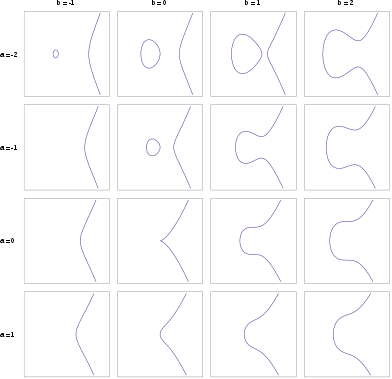
\includegraphics{EC}

        Как можно видеть, имеем 2 разные ситуации: когда график кривой представляет из себя множество, состоящие из одной связной 
        компоненты и из двух. Так же можно видеть, что при некоторый значениях параметров возникают особенности: кривая может пересечь саму себя,
        а так же есть точка излома. Кривые, обладающие такими особенностиями называют вырожденными. Для определения всех этих ситуаций введем
        понятие \textit{дискриминанта}. \textit{Дискриминантом} эллиптической кривой назовем величину 
        $$
            \Delta = -16(4a^3 + 27b^2)
        $$ 
        Если $\Delta < 0$, то кривая имеет две компоненты, если $\Delta > 0$, то кривая имеет одну компоненту. Если же
        $\Delta = 0$, то кривая является вырожденной.

        Далее будем предполагать что кривая является невырожденной, то есть ее дискриминант отличен от нуля. 

        Последнее что нам потребуется это ввести понятие бесконечно удаленной точки. Чтобы не углубляться в науку скажем что это точка, находящаяся где-то
        за пределами плоскости и принадлежащая нашей эллиптической кривой. Таким образом будем рассматривать кривые вида
        $$
            E = \{(x, y) | y^2 = x^3 + ax + b, -16(4a^3 + 27b^2) \neq 0\} \cup \{\infty\}
        $$

    \section{Сложение точек на кривой}
        Сперва определим эту операцию геометрически. Введем понятие нейтрального элемента. Нейтральным элементом назовем точку $\infty$. Рассмотрим 3 точки $P, Q, R' \in E$. Будем говорить что их
        сумма равна нулю, если они лежат на одной прямой. $P + Q + R' = 0$. Чтобы получить именно сумму точек $P$ и $Q$ введем понятие
        обратного элемента. Точкой, обратной к точке $R' = (x_r, y_r)$, назовем точку с координатами $R = (x_r, -y_r)$. 
        
        Заметим, что в определении имеются определенные неточности. Например, что будет если окажется что $P = Q$? Тогда мы будем проводить
        касательную к точке $P$. Что будет если $P = 0$? Тогда чисто формально, $P + Q = 0 + Q = Q$. Что будет если сложить $P + (-P)$? Тогда можно сказать, что
        прямая  проходит через точки $P, -P, \infty$, таким образом $P + (-P) = 0$.

\end{document}